\section{Screening Experiments}
\noindent\rule[\linienAbstand]{\linewidth}{\linienDickeDick}
A production process is usually influenced by many factors. We are now concentrating on an essential factor of the product that
should become the target of our investigations. In order to find the best production condition, we have to know how the essential factors interact.\\
If we want to experimentally investigate the interaction of several factors on the response variable we must observe the process under different production conditions.

\subsection{$\mathbf{2^k}$ Factorial Designs}
\noindent\rule[\linienAbstand]{\linewidth}{\linienDicke}
The number of experiments rapidly increases to an unrealistically large number the more factors are involved. To reduce the number of runs we only use two levels (low and high) per factor.\\

With a $2^k$ factorial design we can efficiently code the different runs by two coding schemes. One is based on $+$ and $-$ signs and the other on lowercase letters. The eight experimental runs for a $2^3$ design based on three factors $A$, $B$ and $C$ are listed in the following table.
\begin{table}[H]
  \centering
  \scriptsize
  \begin{tabular}{c|ccc|c|c}
    Run & \multicolumn{3}{c}{Factors} & Letters & Example\\
      & A    & B    & C               &         & Data\\ \hline
    1 & $-1$ & $-1$ & $-1$            & $( 1)$  & \color{red}  34 \\
    2 & $+1$ & $-1$ & $-1$            & a       & \color{blue} 26 \\
    3 & $-1$ & $+1$ & $-1$            & b       & \color{red}  33 \\
    4 & $+1$ & $+1$ & $-1$            & ab      & \color{blue} 21 \\
    5 & $-1$ & $-1$ & $+1$            & c       & \color{red}  24 \\
    6 & $+1$ & $-1$ & $+1$            & ac      & \color{blue} 23 \\
    7 & $-1$ & $+1$ & $+1$            & bc      & \color{red}  19 \\
    8 & $+1$ & $+1$ & $+1$            & abc     & \color{blue} 18 \\
  \end{tabular}
\end{table}
With a $2^k$ plan it is possible to estimate both the main effects as well as interactions.
\begin{itemize}
  \item The \textbf{main effect of a factor} is the average response value for all test runs at the high level of the factor minus the average response value for runs at the low level of the factor.
  \item The \textbf{two factor interaction effect} is one-half of the difference between the main effects of one factor calculated at the two levels of the other factor.
\end{itemize}

\textbf{Example of main effect}
\begin{equation}
  \begin{split}
    \text{main effect for}\; A &= \frac{1}{4}(\color{blue}26+21+23+18\color{black})-(\color{red}34+33+24+19\color{black})\\
    &= 22.0-27.5 = -5.5
  \end{split}
\end{equation}
\textbf{Example of interaction effect}
\begin{align*}
  \text{mean if}\; A&=-1 \;\text{and}\; C=-1: 33.5 & \text{mean if}\; &A=+1 \;\text{and}\; C=-1: 23.5 \\
  \text{mean if}\; A&=-1 \;\text{and}\; C=+1: 21.5 & \text{mean if}\; &A=+1 \;\text{and}\; C=+1: 20.5
\end{align*}

\begin{equation}
  \begin{split}
    \text{interaction effect}\; A:C &= \frac{1}{2}((33.5-21.5)-(23.5-20.5))\\
    &= \frac{1}{2}(12-3) = 4.5
  \end{split}
\end{equation}

The calculation of the interaction effect can be made simpler by expanding the matrix with additional columns by adding all possible
products between the columns of the matrix.
\begin{table}[H]
  \centering
  \scriptsize
  \begin{tabular}{c|ccc|cccc}
    Run & \multicolumn{3}{c}{Factors} & \multicolumn{4}{c}{Interactions} \\
        & A    & B    & C             & $A:B$ & $A:C$                         & $B:C$ & $A:B:C$  \\ \hline
     1  & $-1$ & $-1$ & $-1$          & $+1$  & $\color{red}+\color{black}1$  & $+1$  & $-1$ \\
     2  & $+1$ & $-1$ & $-1$          & $-1$  & $\color{red}-\color{black}1$  & $+1$  & $+1$ \\
     3  & $-1$ & $+1$ & $-1$          & $-1$  & $\color{red}+\color{black}1$  & $-1$  & $+1$ \\
     4  & $+1$ & $+1$ & $-1$          & $+1$  & $\color{red}-\color{black}1$  & $-1$  & $-1$ \\
     5  & $-1$ & $-1$ & $+1$          & $+1$  & $\color{red}-\color{black}1$  & $-1$  & $+1$ \\
     6  & $+1$ & $-1$ & $+1$          & $-1$  & $\color{red}+\color{black}1$  & $-1$  & $-1$ \\
     7  & $-1$ & $+1$ & $+1$          & $-1$  & $\color{red}-\color{black}1$  & $+1$  & $-1$ \\
     8  & $+1$ & $+1$ & $+1$          & $+1$  & $\color{red}+\color{black}1$  & $+1$  & $+1$ \\
  \end{tabular}
\end{table}
For instance, the column of the interaction $A:B$ is obtained by multiplying the columns of the factors $A$ and $B$. The interaction effect can then alternatively be calculated as follows:

\begin{equation}
  A:C = \frac{1}{2^{3-1}}(
  \color{red}+\color{black}34
  \color{red}-\color{black}26
  \color{red}+\color{black}33
  \color{red}-\color{black}21
  \color{red}-\color{black}24
  \color{red}+\color{black}23
  \color{red}-\color{black}19
  \color{red}+\color{black}18
  ) = 4.5
\end{equation}

The number of $8$ runs with a $2^3$ design only allows us to calculate point estimates of the effects. There are no degrees of freedom left for the residuals and it is not possible to perform statistical tests. More than one measurement in each test situation is needed (Most often too expensive) in order to find out which effects are significantly different from zero. In R this analysis can then be done with the $\texttt{aov}$ command.\\

If only one measurement is made in each test situation, then we can estimate all the main and interaction effects, but not test them for significance (i.e. test the null hypothesis that the individual effects are zero). Nevertheless, there is a possibility to identify significant effects.\\
If most of the effects are zero, then the estimated effects will only detect noise due to the measurement error and therefore vary randomly around zero. If all the estimated effects are considered as realisations of the same noise, then we can graphically analyse them with a q-q plot. The significant effects, which are not noise at all, will then show up as outliers. The quantile of the $i$th ordered observation can be calculated
according to the formula
\begin{equation}
  q_i = \frac{1}{2} + \frac{1}{2}\frac{i - \frac{3}{8}}{e + \frac{1}{4}},
\end{equation}
where $e$ denotes the number of estimated effects.
\begin{table}[H]
  \setlength{\tabcolsep}{0.0em}
  \scriptsize
  \begin{tabular}{p{\linewidth / 2 - 0.5em}@{\hskip 1em}p{\linewidth / 2 - 0.5em}}
    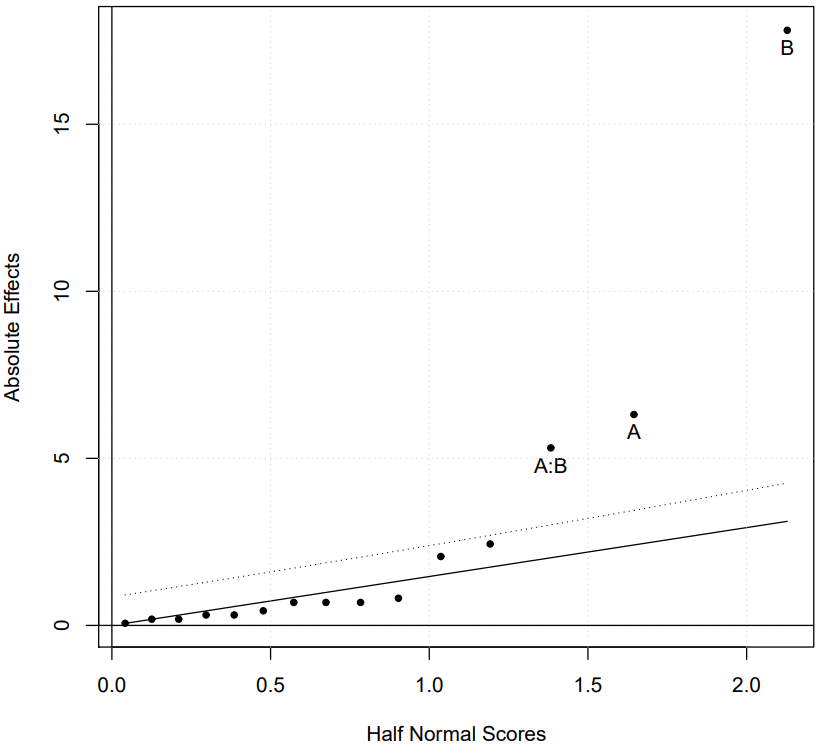
\includegraphics[width=\linewidth]{Pics/14.1.2.png}& 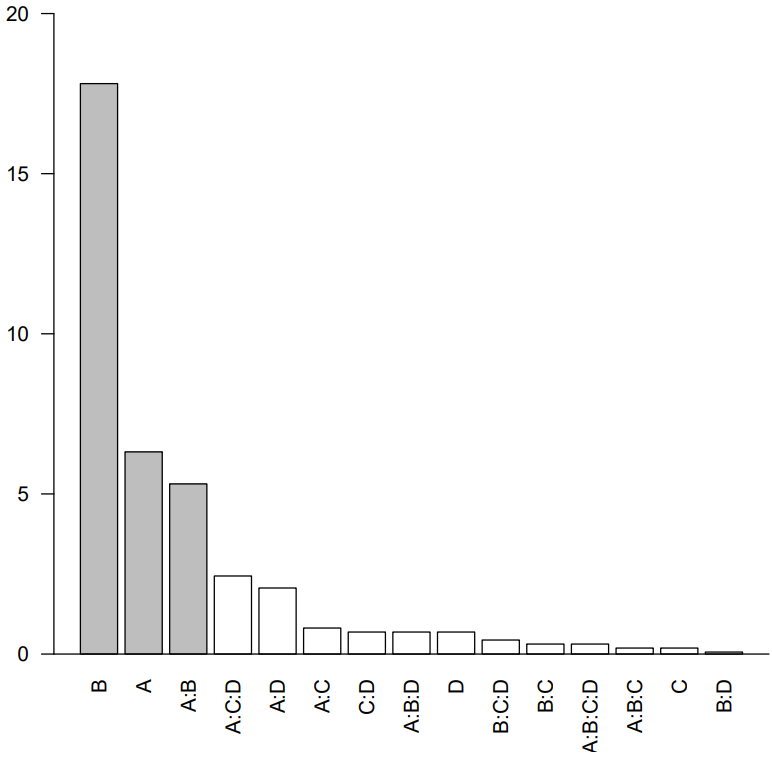
\includegraphics[width=\linewidth]{Pics/14.1.3.png} \\
    Half normal plot of the estimated main and interaction effects. The non-significant effects vary around the diagonal solid line and are below the dotted line. The significant effects are labeled with the name of the factor. &
    Pareto Chart. The significant main effects $A$ and $B$ and the interaction effect $A:B$ (gray) clearly dominate the non-significant effects (white).
  \end{tabular}
\end{table}
\subsection{$\mathbf{2^k}$ Fractional Factorial Designs}
\noindent\rule[\linienAbstand]{\linewidth}{\linienDicke}
Few major effects and few interaction effects are significant. The more factors examined, the smaller the ratio between the number of major effects and the number of interactions. With six factors, it has one intercept, six major effects and 57 interaction effects, i.e. only 9.4\% major effects. The remaining 90.6\% of the effort is needed to estimate the interaction effects, many of which are not significant or relevant. Thus, in screening experiments, complete $2^k$ designs are rather inefficient for large $k$, which is why so-called $2^k$ fractional factorial designs are used.\\

Fractional factorial designs are created by replacing some of the higher-order interaction with additional experimental factors. Because the interaction effect of the highest order is most likely to be insignificant, the corresponding column in the following table, i.e. the column A:B :C
is now assigned to a new main effect D.
Because only half of the runs need to be measured compared to a full $2^4$ design, this is called a $2^{k-1}$ fractional factorial design. The advantage of using fractional factorial designs is a significant reduction of the number of runs required.\\

The effects $D$ and $A:B:C$ are called confounded or aliased in such a situation. The reason to alias $D$ with $A:B:C$ is first of all that we speculate that the effect $A:B:C$ is negligible. If so, we get an estimate of the main effect $D$ with only 8 runs.
The entire set of aliases in a fractional factorial design is called alias structure of the design.

\begin{table}[H]
  \centering
  \scriptsize
  \begin{tabular}{ccc}
    Effect & & Alias \\
    $I$  & $=$ & $ABCD$  \\
    $A$  & $=$ & $BCD$   \\
    $B$  & $=$ & $ACD$   \\
    $C$  & $=$ & $ABD$   \\
    $D$  & $=$ & $ABC$   \\
    $AB$ & $=$ & $CD$    \\
    $AC$ & $=$ & $BD$    \\
    $AD$ & $=$ & $BC$    \\
  \end{tabular}
\end{table}
The alias structure can be summarised as follows:
\begin{itemize}
  \item Each main effect is aliased with a three-factor interaction.
  \item All two factor interactions are aliased with one another.
  \item The single four-factor interaction is aliased with the grand mean of the data.
\end{itemize}
